\section{Wprowadzenie do analizy składniowej ALL(*)}
W tej sekcji opisano idee i intuicje dotyczące analizy składniowej ALL(*).
Następnie w sekcji 5 przedstawiono algorytm bardziej formalnie.
Moc strategii zstępującej analizy składniowej jest związana ze strategią wyboru
alternatywnej produkcji do rozwinięcia bieżącego symbolu nieterminalnego.
W przeciwieństwie do parserów LL(k) i LL(*), parsery ALL(*) zawsze wybierają
pierwszą alternatywę z tych która prowadzi do prawidłowej analizy składniowej.
Wszystko nie lewostronnie rekurencyjne gramatyki są zatem ALL(*).
\par
Zamiast polegać na statycznej analizie gramatyki,
parser ALL(*) adaptuje się do zdań wejściowych przedstawionych w czasie parsowania.
Parser analizuje bieżący punkt decyzyjny (symbol nieterminalny przy wielu produkcjach)
używając mechanizmu GLR, aby zbadać wszystkie możliwe ścieżki decyzyjne
w odniesieniu do bieżącego „stosu wywołań” wewnątrz-procesowych symboli nieterminalnych,
a pozostałe dane wejściowe na żądanie. Analizator stopniowo i dynamicznie
tworzy jeden automat lookahead DFA na jedną decyzję, który zapisuje mapowania
z sekwencji lookahead na numer przewidywanej produkcji.
Jeśli utworzone DFA pasuje do bieżącego lookahead, parser może ominąć analizę
i natychmiast rozwinąć przewidzianą alternatywę.
Opisane badania w Sekcji 7 wskazują, że parsery ALL(*) zazwyczaj wykorzystują
DFA istniejące w już w cache a te DFA mają decydujące znaczenie dla wydajności. 

\begin{figure}[!ht]
\noindent\rule{\linewidth}{0.3pt}
\lstset{language=Java,
                basicstyle=\ttfamily,
                keywordstyle=\color{blue}\ttfamily,
                stringstyle=\color{magenta}\ttfamily,
                commentstyle=\color[rgb]{0,0.3,0}\ttfamily
}
\begin{lstlisting}
void stat() { // parse according to rule stat
	switch ( adaptivePredict("stat", call stack)) {
		case 1 : // predict production 1
			expr(); match('='); expr(); match(';');
			break ;
		case 2 : // predict production 2
			expr(); match(';'); break ;
	}
}
\end{lstlisting}
\noindent\rule{\linewidth}{0.3pt}
\caption{Rekurencyjnie zstępujący kod dla star gramatyki Ex}
\end{figure}


\begin{figure}[h]
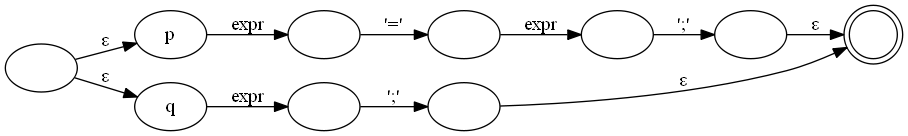
\includegraphics[width=0.9\textwidth]{Figure3.png}
\caption{ATN dla reguły ANTLR stat w gramatyce Ex}
\end{figure}
\par
Ze względu na fakt, iż ALL(*) różni się od deterministycznych zstępujących
metod tylko w mechanizmie przewidywania, możemy utworzyć konwencjonalne parsery
rekurencyjne LL, ale z istotnym wyróżnikiem.
Parsery ALL(*) wywołują specjalną funkcję przewidywania, adaptivePredict,
która analizuje gramatykę w celu utworzenia automatu lookahead DFA
zamiast po prostu porównywać lookahead z statycznie obliczonym zbiorem symboli.
Funkcja adaptivePredict przyjmuje symbole nieterminalne i stos wywołań parsera
jako parametry i zwraca przewidziany numer produkcji lub zgłasza wyjątek,
jeśli nie ma żadnej wykonalnej produkcji. Na przykład, reguła stat z przykładu
w Sekcji 2.1 odzwierciedla analizę składniową przedstawioną na Rysunku 2.
\par
Przewidywanie ALL(*) ma podobną strukturę do znanego algorytmu budowy
podzbióru NFA-to-DFA. Celem jest wykrycie zbioru stanów, które parser może
osiągać po obejrzeniu niektórych lub wszystkich pozostałych danych wejściowych
w stosunku do obecnej decyzji. Podobnie jak przy  tworzeniu podzbiorów,
stan DFA ALL(*) jest możliwym zbiorem konfiguracji parsera po dopasowaniu
danych wejściowych prowadzących do tego stanu. Zamiast NFA jednak, ALL(*) symuluje
działania rozszerzonej rekurencyjnej sieci przejść (ATN) [27]
odzwierciedlając gramatykę, gdyż ATNs ściśle odzwierciedlają strukturę gramatyki.
\par
(ATNs wyglądają podobnie jak diagramy składniowe, które mogą posiadać działania
i semantyczne predykaty). Statyczna analiza LL(*) również operuje na ATN z tego
samego powodu. Rysunek 3 przedstawia podautomat ATN dla reguły stat.
Konfiguracja ATN reprezentuje stan wykonania subparsera i śledzi stan ATN,
przewidziany numer produkcji, oraz stos wywołań subparsera ATN: krotka (p, i, $\gamma$).
1 Konfiguracje obejmują numery produkcji, tak więc przewidywanie może identyfikować
która produkcja pasuje do bieżącego lookahead.
W przeciwieństwie do analizy statycznej LL(*), ALL(*) stopniowo buduje DFA,
biorąc pod uwagę tylko sekwencje lookahead, zamiast wszystkich możliwych sekwencji.

\begin{figure}[h]
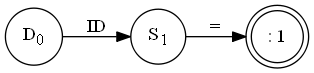
\includegraphics[width=0.32\textwidth]{Figure4a.png}
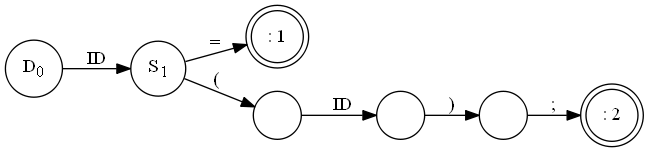
\includegraphics[width=0.64\textwidth]{Figure4b.png}
\\
(po lewo) Po x=y;\\
(po prawo) Po x=y; i f(x);
\caption{Przewidujące DFA dla decyzji stat}
\end{figure}
\par
Gdy analiza składniowa podejmuje decyzję po raz pierwszy, adaptivePredict
inicjuje lookahead DFA dla tej decyzji poprzez utworzenie stanu DFA, $D_0$.
$D_0$ jest zbiorem konfiguracji subparser ATN osiągalnym bez wykorzystywania
początkowego symbolu wejściowego w każdej lewej stronie produkcji.
Na przykład, tworzenie $D_0$ dla nieterminali stat na Rysunku 3 rozpoczyna się
od dodania konfiguracji ATN (p; 1; []) i (q; 2; []) gdzie p i q są stanami
ATN analogicznymi dla produkcji 1 i 2 lewych stron, a [] jest pustym stosem wywołań dla subparsera
(jeśli stat jest symbolem początkowym).
\par
Analiza następnie oblicza nowy stan DFA, wskazując gdzie symulacja ATN może
być osiągalna po wykorzystaniu pierwszego symbolu lookahead, po czym łączy
dwa stany DFA krawędzią oznaczoną tym symbolem. Analiza postępuje,
dodając nowe stany DFA, aż wszystkie konfiguracje ATN w nowo utworzonym
stanie DFA przewidują taką samą produkcję: (-; i; -).
Funkcja adaptivePredict uznaje ten stan za akceptowalny i powraca do parsera
z tą liczbą produkcji. Rysunek 4a przedstawia lookahead DFA dla decyzji stat,
po tym jak adaptivePredict przeanalizował zdania wejściowy x = y;.
DFA nie posiada wglądu poza = ponieważ = jest wystarczające, aby jednoznacznie
rozróżnić wyrażenie produkcji. (Zapis: 1 oznacza „przewidywaną produkcję 1”).
\par
Najczęściej adaptivePredict odnajduje istniejący DFA dla konkretnej decyzji.
Celem jest znalezienie lub utworzenie ścieżki poprzez DFA do akceptowalnego stanu.
Jeśli adaptivePredict osiągnie (nieakceptowalny) stan DFA bez krawędzi
dla bieżącego symbolu lookahead, powraca do symulacji ATN aby rozszerzyć DFA
(bez odwijania danych wejściowych). Na przykład, do analizy drugiej frazy
danych wejściowych dla stat, takich jak f(x);, adaptivePredict znajduje
istniejącą krawędź ID z $D_0$ i przeskakuje do $s_1$ bez symulacji ATN.
Nie ma żadnego istniejącej krawędzi z $s_1$ dla lewego nawiasu, tak więc analiza
symuluje ATN aby zakończyć ścieżkę do akceptowalnego stanu,
który przewiduje drugą produkcję, zgodnie z Rysunkiem 4b.
Należy zauważyć, że z faktu iż sekwencja ID (ID) przewiduje obie produkcje,
analiza postępuje dotąd aż DFA będzie posiadać krawędzie dla symboli = i;.
\par
Jeśli symulacja ATN oblicza nowy stan docelowy, który już istnieje w DFA,
symulacja dodaje nową krawędź nakierowując istniejący stan i przełączając się
na tryb symulacji DFA, począwszy od tego stanu. Wskazywanie jako cel Istniejących
stanów powoduje że w DFA mogą pojawiać się cykle.
Rozszerzanie DFA do obsługi nieznanych fraz empirycznie zmniejsza
prawdopodobieństwo przyszłych symulacji ATN, tym samym zwiększając szybkość
analizy składniowej (Część 7). 
